% Name: Electromagnetic wave
% Description: A plane electromagnetic wave traveling along x: the electric field E oscillating in the vertical plane and the magnetic field B in the horizontal plane, in phase and at right angles.
% Tags: electromagnetic wave, electric field, magnetic field, light

\usetikzlibrary{arrows.meta}

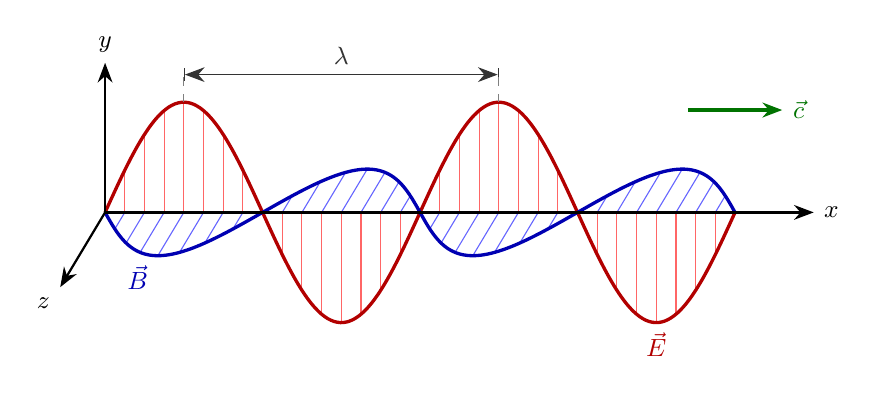
\begin{tikzpicture}[>={Stealth[length=2.5mm]}, x={(1cm,0)}, y={(0,1cm)}, z={(-0.3cm,-0.5cm)}, every node/.style={font=\small}]
  % E = 1.4 sin(2 pi x / 4) along y and B = 1.1 sin(2 pi x / 4) along z, so E x B points along x.
  \foreach \x in {0.25,0.5,...,8} {
    \draw[red!60, thin] (\x,0,0) -- (\x,{1.4*sin(90*\x)},0);
    \draw[blue!60, thin] (\x,0,0) -- (\x,0,{1.1*sin(90*\x)});
  }
  \draw[very thick, red!70!black, domain=0:8, samples=100, smooth] plot (\x, {1.4*sin(90*\x)}, 0);
  \draw[very thick, blue!70!black, domain=0:8, samples=100, smooth] plot (\x, 0, {1.1*sin(90*\x)});
  \draw[->, thick] (0,0,0) -- (9,0,0) node[right] {$x$};
  \draw[->, thick] (0,0,0) -- (0,1.9,0) node[above] {$y$};
  \draw[->, thick] (0,0,0) -- (0,0,1.9) node[below left] {$z$};
  \node[red!70!black, below] at (7,-1.4,0) {$\vec{E}$};
  \node[blue!70!black, below left] at (1,0,1.1) {$\vec{B}$};
  \draw[|<->|, gray!40!black] (1,1.75,0) -- node[above] {$\lambda$} (5,1.75,0);
  \draw[dashed, gray] (1,1.4,0) -- (1,1.75,0) (5,1.4,0) -- (5,1.75,0);
  \draw[->, very thick, green!45!black] (7.4,1.3,0) -- ++(1.2,0,0) node[right] {$\vec{c}$};
\end{tikzpicture}
